\subsubsection{2.3.5.03 LLNL ATDM SW Ecosystem \& Delivery: DevRAMP}

\paragraph{Overview}
The {\bf DevRAMP} (Reproducibility, Analysis, Monitoring, and Productivity
for Developers) is creating tools and services that multiply the
productivity of HPC developers through automation. The project has two
major software efforts:

\begin{enumerate}
    \item {\bf Spack} is a package manager for
    HPC~\cite{melara+:cug17,gamblin+:sc17-spack-tutorial,gamblin+:sc16-spack-tutorial,gamblin+:sc15,gamblin+:llnl-spack-tutorial-17,gamblin+:ecp18-spack-tutorial,gamblin:pp18-spack,gamblin:hpckp17,gamblin:fosdem18-compilers,gamblin:fosdem18-binary,gamblin:ecp18-spack-sotu,gamblin:eb-user-meeting18,becker+:hust16}. It
    automates the process of downloading, building, and installing
    different versions of HPC software packages and their dependencies.
    With Spack, facilities can manage complex, multi-user software
    deployments on supercomputers, and developers can keep their own
    dependencies up to date in a single-user environment. Spack enables
    complex applications to be assembled from components, lowers barriers
    to software reuse, and allows complex HPC environments to be
    reproduced easily. It is the glue that holds the ECP software
    ecosystem together.

    \item {\bf Sonar} is a data cluster and a software stack for
    performance monitoring and analysis. Sonar allows developers and
    facility staff to understand how supercomputers and applications
    interact. The system continuously aggregates data from system-level
    monitoring services, application-level measurement tools, and
    facility power and temperature meters.  Any facility user can log in,
    examine performance data and other data collected about their HPC
    jobs, and share it with other users. Our focus is on security for the
    services running on Sonar (e.g., JupyterHub), and on developing an
    easy-to-use query tool, which we call ScrubJay.
\end{enumerate}


\paragraph{Key  Challenges}
{\it Spack} makes HPC application complexity manageable. HPC simulation
codes are notoriously complicated, and installing a code on a new
platform is not a simple task.  Codes are not self-contained; they rely
on tens or even hundreds of {\it dependencies} to implement their
functionality. While dependencies allow us to leverage the work of others
through code reuse, integrating hundreds of dependencies in the same
application is a monumental challenge.  Dependencies may require
different configurations and versions of their own dependency libraries,
and codes must be built and tested with different implementations of
interfaces MPI, BLAS, and LAPACK. The space of possible builds is
combinatorial in size, and it can only be effectively managed through
automation.

{\it Sonar} aims to find the root causes of performance variability of
jobs that run at Livermore Computing.  A single application execution may
have a different runtime depending on the system it runs on, the file
system it uses, or other jobs running at the same time.  A single
application execution may not accurately characterize performance.  The
causes of this variability may include file system performance, per-node
power consumption, application code performance, and even processor
performance from node to node. To analyze and understand performance
variability, we must collect data from the HPC center {\it and} from jobs
running at the facility, but we cannot show all application- and
facility-level data to all users. We need hardened security and
fine-grained permissions to ensure that data on Sonar is kept safe.

\paragraph{Solution Strategy}
{\it Spack} addresses HPC software complexity in three ways. First, it
provides a powerful build system and a domain-specific language for
writing package recipes.  This allows HPC builds to be templated and
easily mapped to HPC architectures. It provides dependency resolution
infrastructure, including virtual dependencies, a full parameter system,
and a dependency resolver we call a {\it concretizer}. Together, these
allow developers to specify customize builds for their own environments
based on {\it abstract} descriptions, while Spack handles the tedious
aspects of integrating with a new machine. Finally, Spack is an online
service where package recipes can be shared and the HPC community can
leverage each others' effort to reuse software. One of Spack's greatest
strengths is its very active online contributor community.

{\it Sonar} is a data cluster, a data model, a set of monitoring tools,
and an analysis front-end for manipulating this data. To deploy this in
the Livermore Computing (LC) center, our project has focused on securing
all components of this stack so that they can be hosted as services in a
multi-tenant environment. We have deployed the Cassandra database, the
Spark parallel processing engine, a custom tool of our own called
ScrubJay, among other components. We have added integration that allows
each tool to use LC's user ids and groups with access control lists. In
the case of Jupyter Notebooks and other services that launch jobs, we are
also hardening the process launch infrastructure so that notebooks launch
on behalf of users run {\it as} those users in the LC environment.

\paragraph{Recent Progress}
Figure~\ref{fig:sonar-spack} (left) shows the progress so far on Sonar
deployment.  The Cassandra database, as well as data collection from
compute clusters, filesystems, and facility temperature data is complete.
We have also recently completed a full-center deployment of JupyterHub
for accessing the data in the cluster. We were able to deploy JupyterHub
by adding SSL encryption to links between the hub and each notebook; this
required us to build a custom certificate authority into JupyterHub.  We
are currently preparing to upstreaming our solution to the mainline
JupyterHub repository.
\begin{figure}[htb]
    \centering
    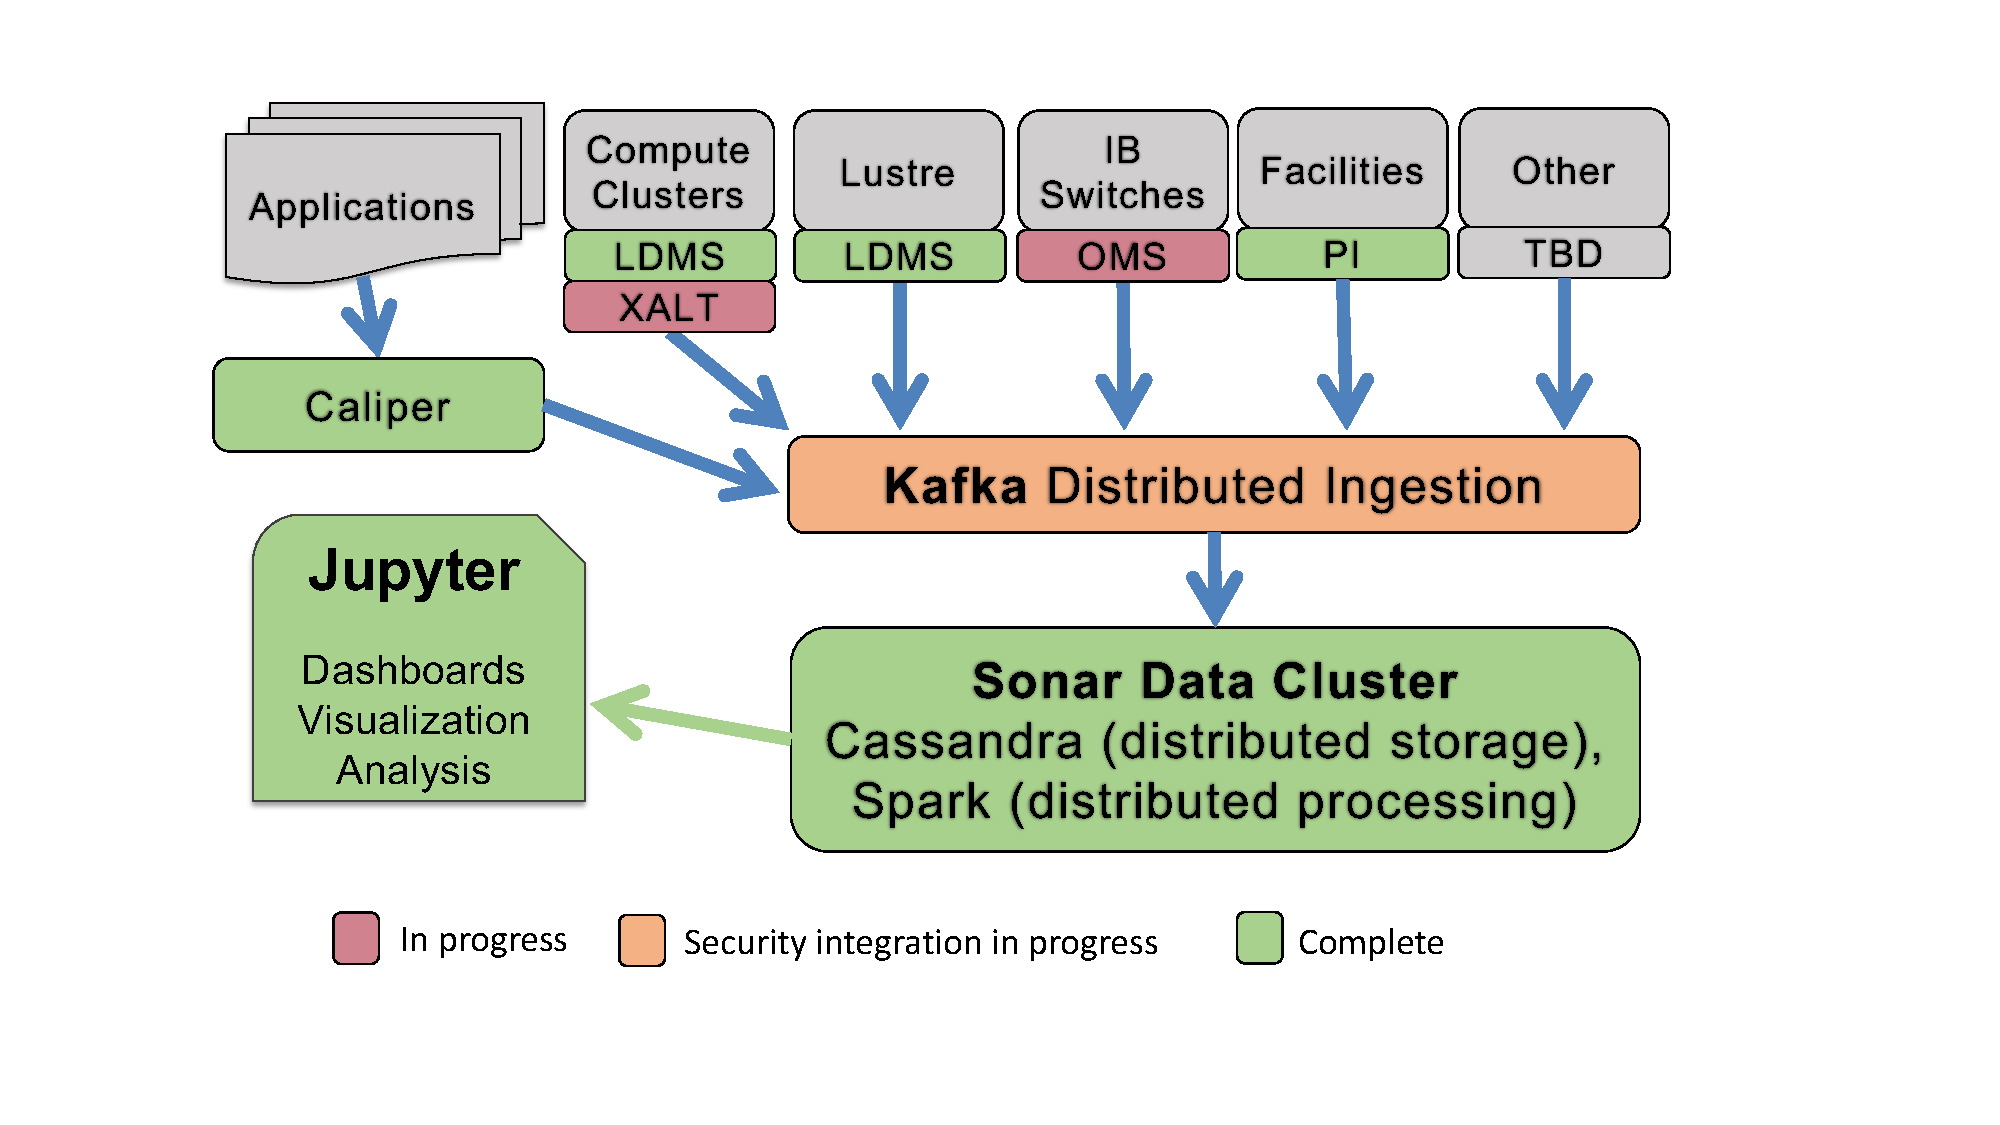
\includegraphics[height=1.5in]{projects/2.3.5-Ecosystem/2.3.5.03-LLNL-ATDM-Ecosystem/sonar}~~~~~~~
    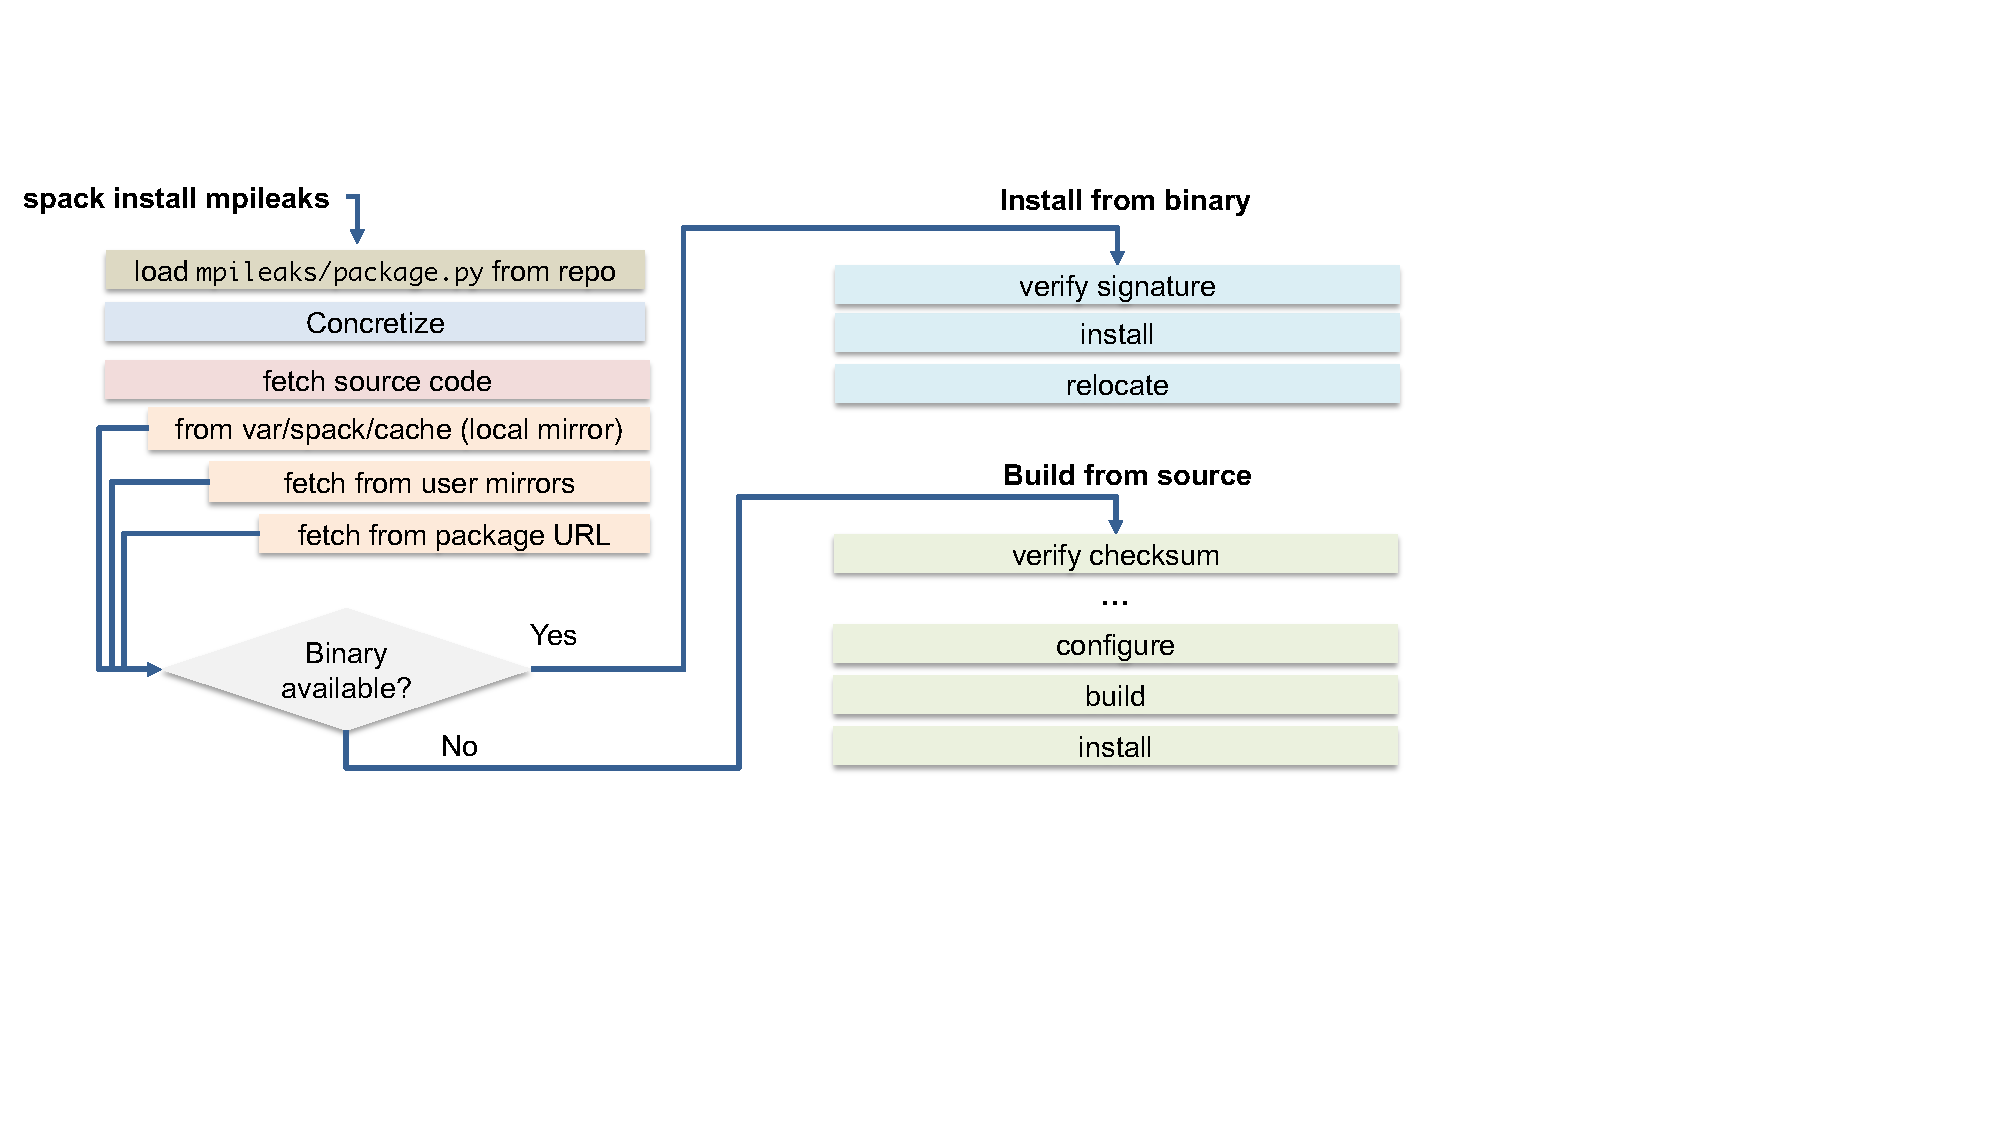
\includegraphics[height=1.5in]{projects/2.3.5-Ecosystem/2.3.5.03-LLNL-ATDM-Ecosystem/spack-fetch}
    \caption{
        \label{fig:sonar-spack} Sonar deployment (left) and
        Spack binary packaging (right).
    }
\end{figure}

We recently added the capability to create relocatable binary packages to
Spack~(Figure~\ref{fig:sonar-spack}, right).  Spack typically builds all
of its packages from source, as this is the de-facto software
distribution method for HPC systems. Recent additions to Spack allow us
to package even HPC software in optimized binary form, and to install in
minutes what could previously take hours. We are currently working on
making Spack's dependency resolution algorithm more robust to handle more
aggressive use of binary packages. Figure ~\ref{fig:concretize} shows the
current Spack concretizer, which will only reuse binaries that exactly
match a client-side concrete spec. The new version will allow Spack to
consider available remote binaries at install time, and to search more
aggressively through available binaries for usable dependencies. This
will mean even less rebuilding of software, and for HPC systems, this
means we will be able to match optimized binaries to the machine.

\begin{figure}[htb]
    \centering
    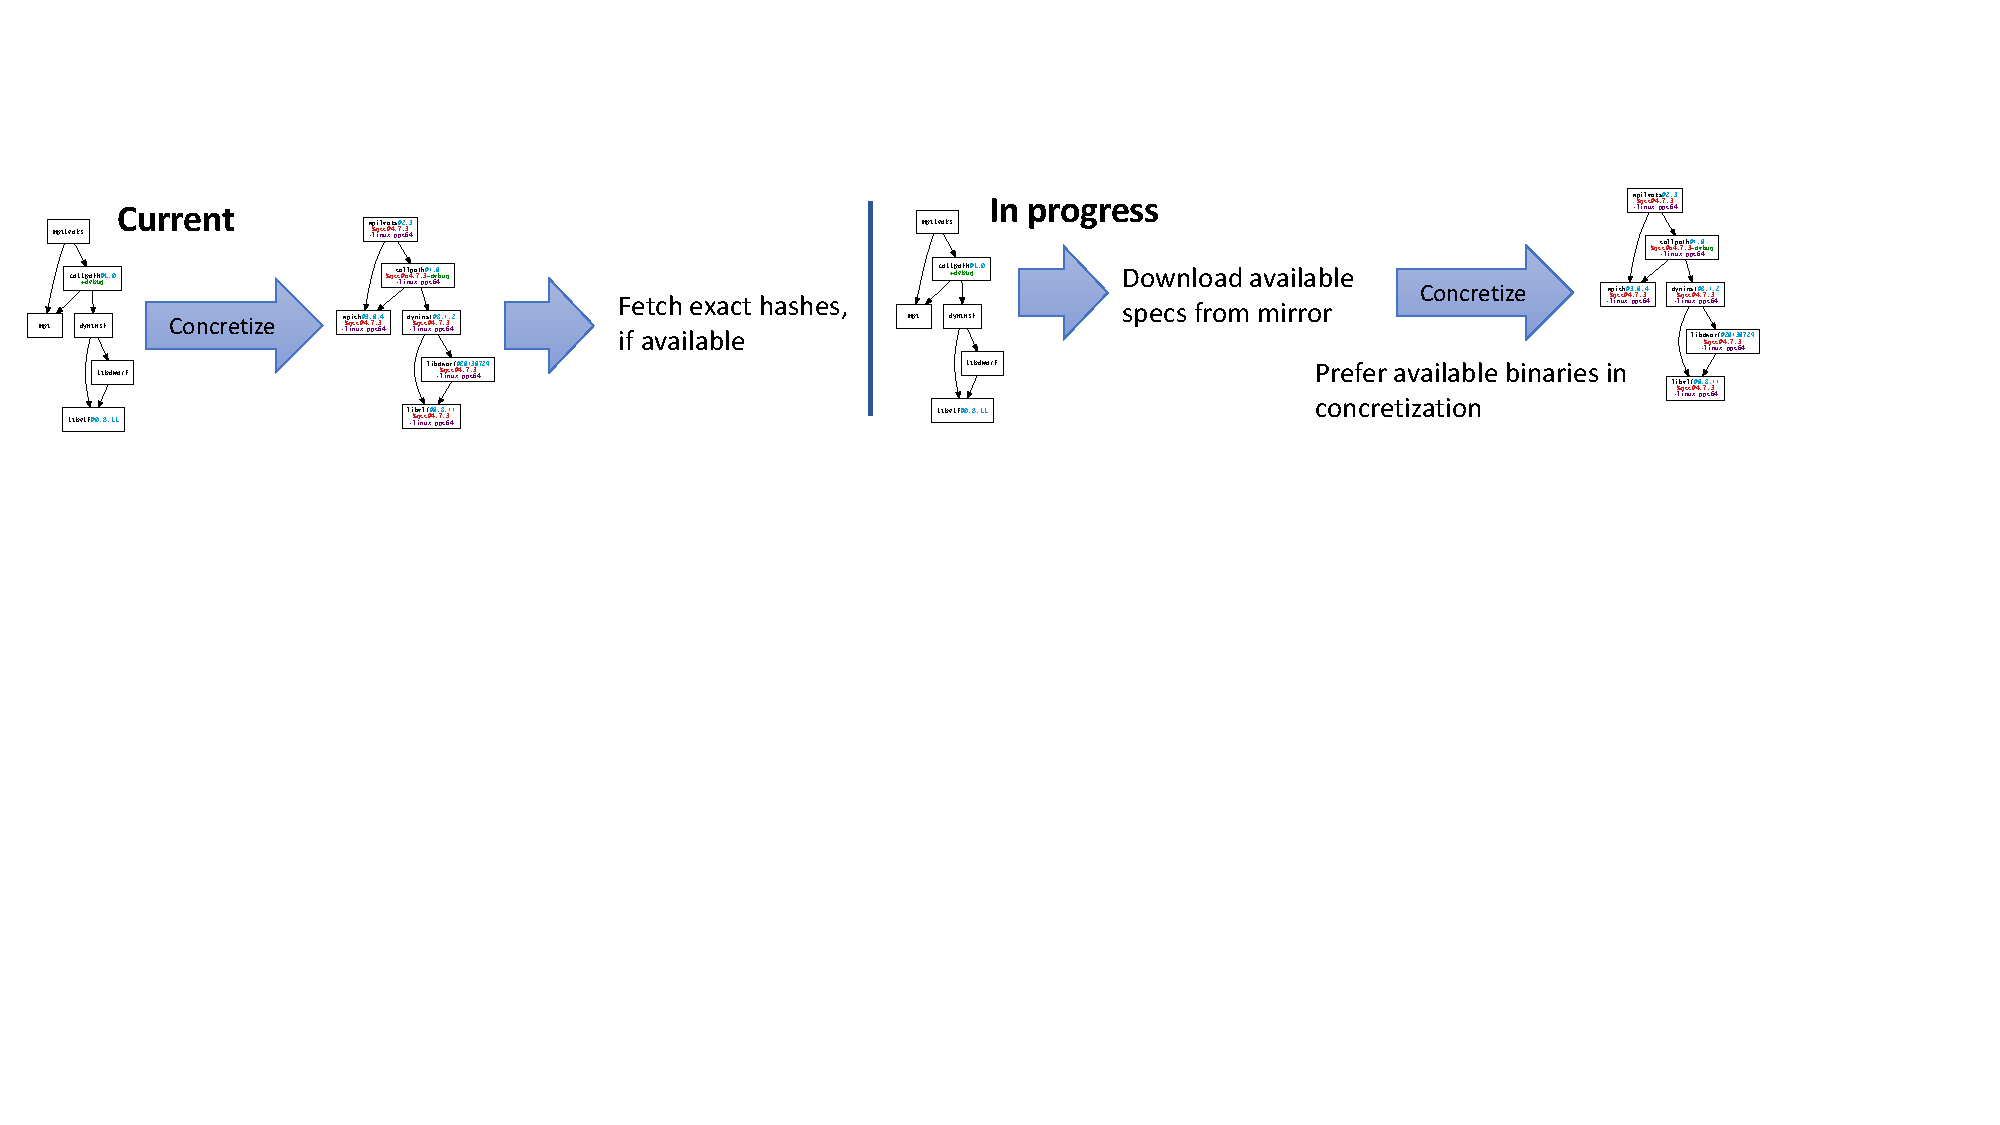
\includegraphics[width=\textwidth]{projects/2.3.5-Ecosystem/2.3.5.03-LLNL-ATDM-Ecosystem/spack-concretizer}
    \caption{\label{fig:concretize}
        Spack concretizer design changes.
    }
\end{figure}


\paragraph{Next Steps}
\begin{enumerate}

    \item {\bf Securing Kafka for Sonar.}  Sonar will ingest application
    data from the filesystem using a tool called Kafka. Kafka is a
    streaming communication infrastructure; it runs as a daemon and
    reliably transfers data from files to a database.  Kafka typically
    runs as a single user, but HPC centers are multi-tenant
    installations.  We will be adding functionality to ensure that Kafka
    preserves the identity of file owners in the filesystem when it
    ingests data into the database.

    \item {\bf Spack release testing and binary hosting.} Spack serves as
    a repository for package recipes, but we do not have any automated
    build testing of packages included in the Spack repository.  To
    increase the robustness and reliability of Spack, we are adding
    automation for building all packages in each Spack release, and for
    creating binary packages from such builds. We aim to provide binary
    packages for common configurations of Spack packages.
\end{enumerate}
